The headline of news is a summary of its body content and most of the time, it carries valuable data. So, we focused on detecting the news headlines stance towards claim(H2C), as well as the news articles stance towards a claim(B2C). According to the lower amount of text in the news headline, most of the experiments are firstly applied to H2C. Then, better approaches are applied to A2C.  
\section{Preprocessing}
The first and mandatory preprocessing step is to tokenize words in the corpus in order to remove and detect special words. Four different following tokenizer performance on Persian language has been evaluated. 
\begin{itemize}
	\item \textbf{Hazm\footnote{\label{fn:hazm}sobhe.ir}:}
	Hazm is a python library Persian language processing tool kit. It has variety of functions such as word and sentence tokenizer, word lemmatizer, POS tagger, Shallow, and Dependency parser. \textit{Hazm} tokenizer is \textit{NLTK} compatible\footref{fn:hazm}.
	
	\item \textbf{NLTK\footnote{nltk.org}:}
	NLTK (Natural Language ToolKit)) is a python platform to work easier with human language data. This tool kit supports more than 50 datasets and supports numerous languages including Persian. 
	
	\item \textbf{Stanford\footnote{stanfordnlp.github.io/stanza}:}
	Stanford NLP tools is also another advantageous NLP tools package that is currently switched to \textit{Stanza}. It is efficient for linguistic analysis and supports more than 70 human languages and releases new versions constantly.
	
	\item \textbf{BERT\footnote{huggingface.co/transformers/main\_classes/tokenizer.html}:}
	BERT (\cite{bert}) is a transformer-based machine-learning model which is currently used in various natural language processing tasks. Persian pre-trained BERT model\footnote{huggingface.co/HooshvareLab/bert-base-parsbert-uncased} can be used for tokenizing corpus too. 
\end{itemize}

It is vital in the tokenizing step to break the corpus into correct words. It may happen that tokenizers generate meaningless words, this is why tokenizers limit the number of accepted words. Also, sometimes tokenizers haven't seen words before, and omit them while tokenizing the corpus. According to stated reasons, it is important to choose a tokenizer carefully.


After tokenization, a list of punctuation and Persian stop-words are considered as \textit{denied} and will remove from the corpus in this step. Firstly, the same stop-words was used which have been used by \cite{stance_persian}. After reviewing preprocessed corpus, it was hard to infer the stance from text pieces. So we chose stop-words carefully in a way not to lose refuting or supporting expressions. Kharazi\footnote{\label{fn:kharazi}github.com/kharazi/persian-stopwords} has classified Persian stop-words into verbal, nonverbal, and short. Verbs carry valuable information in news. Nonverbal stop-word class is a better choice to remove low-value words in this task. Besides adding and removing some words in news fields are evaluated against Kharazi's\footref{fn:kharazi} gathered stop-words. 

Also English number characters will remove from the corpus before tokenizing. After preprocessing tokens, all tokens will be concatenated with a space character and considered as prepossessed and clean corpus.


\section{Word Representation}
To represent a corpus, tokens should be converts to vectors. Good vectors have to carry semantic of each word or n-grams, sequential words contents, and be as brief as possible. As a baseline three different Bag-of-word (\cite{bow}), TF-iDF (\cite{tfidf}), and Word-to-Vector (\cite{word2vec}) algorithms are evaluated against each other. More details are explained below.

\subsection{BoW\protect\footnote{en.wikipedia.org/Bag-of-words\_model}}
Bag-of-Words (\cite{bow}) model, is a way to represent texts. BoW keeps words frequency and
dismisses word's orders. Dimension of text representation is equal to the number of specified words plus one for words that don't exist in BoW dictionary. Each cell in output text representation stands for a specific word and the value of that cell is equal to the repetition times of that word in the particular text. As an alternative, it is possible to choose n-gram instead of a single word as BoW dictionary. This may improve BoW model performance in order to keep longer expression semantic but on the other hand dimension of representation exceed vastly. One disadvantage of BoW is it doesn't specify any relation between words with similar semantic meanings. 

\subsection{TF-IDF}

Term Frequency–Inverse Document Frequency (\cite{tfidf}) is an algorithm to present the importance of each word in a corpus in a statistical way. According to the repetition of a specific word in each document and inverse effect of the number documents that the word appears in, a float number will be assigned to each word in that corpus.  
\begin{itemize}
	\item \textbf{Trem frequency (TF):} This item represents how many times a word is used in each document. \textit{TF} should be calculated for each document separately. \textit{TF} term calculate from equation \ref{eq:tf}
	\begin{equation}
	\label{eq:tf}
		tf \left(t,D\right) = \frac{f_{t,d}}{\Sigma_{t^{`} \in d } f_{t^{`}, d}}
	\end{equation}
	
	\item \textbf{Inverse Document Frequency (iDF):} This term presents how much information a word has. The less repetition of a word through documents, the more information it has. This term is calculated from equation \ref{idf}. 
	\begin{equation}
	\label{idf}
		idf \left( t,D\right) = \log \frac{N}{\left|\{d\in D, t \in d\}\right| }
	\end{equation}
\end{itemize}

\noindent
After calculating \textit{TF} and \textit{iDF}, TF-iDF value for each word calculates from equation \ref{tfidf}.
\begin{equation}
	\label{tfidf}
	tf-idf\left(t,d,D\right) =  tf \left( t,D\right) . idf \left( t,D\right)
\end{equation}


\subsection{W2V\protect\footnote{en.wikipedia.org/wiki/Word2vec}}
Word2vec (\cite{word2vec}) is a neural network-based model which learns each word semantic and even it can recommend words with similar meaning to a specific word. Word2Vec represents each word with a vector instead of a number. After the training phase, each word vector serves numbers that are generally similar to words with similar meaning, and words with less correspondence have lower vector similarities. This vector is called word-embedding. It is necessary to have a large corpus in order to train a powerful model which can predict each word vector precisely. Multiple alternative algorithms for Word2Vec exist. In this project, FastText\footnote{fasttext.cc} Word2Vec model is used with vector lengths equal to 300 which is trained on Persian Wikipedia website. Fasttext is an extension of Word2Vec model which treats each word as concatenated n-grams.  


\section{Features}
\label{sec:features}
In machine learning algorithms, feature engineering can be considered the most important step because the desired model trains patterns only corresponding to predictors. Extracting sufficient predictors as compact as possible to having the best predicting accuracy and time-efficient	, requires numerous trials and errors. In the following part of this section, extracted features are explained in detail.
\subsection{Similarity}
The similarity score is offered by \cite{stance_persian}. This feature calculates how much a claim is similar to a headline or a news article, depends on the task. Three following sequence matching score is considered for this feature by utilizing \textit{difflib}\footnote{docs.python.org/3/library/difflib.html} python library.

\begin{itemize}
	\item Ratio: Similarity score in float range 0,1. This parameters calculates from equation \ref{eq_ratio}
	\begin{equation}
		\label{eq_ratio}
		ratio = \frac{2.0 * M}{T}
	\end{equation}
	where:
	\begin{eqexpl}[25mm]
		\item{$T$}Number of elements in both sequences.
		\item{$M$}Number of matches.
	\end{eqexpl}
	\item Quick Ratio: This parameter estimates an upper bound on the Ratio.
	\item Real Quick Ratio: This parameter estimates an upper bound on the Ratio.
\end{itemize}
\subsection{Root Distance}
This feature is suggested by \cite{stance_persian}. Root Distance stands for the distance between the root of a headline and some collected hedge, refuting and reporting words. Firstly, a set of words considered as mentioned group are gathered, and then for each word distance is calculated.
%\newline{\color{red}=================TODO========================}
\subsection{ImportantWords}
List of a controversial and challenging words in news  gathered by \cite{stance_persian} and considered as \textit{important-words}. This feature is a zero-based list with the length of important words, and each cell stands for one word in \textit{important-words}. The list carries the number of repetitions of desire words in a specific news article.
\subsection{Is Question}
Is-Question identifies whether a claim or headline of a news article ends with question marks or not. \cite{stance_persian} dataset contains a column dedicated to this feature.
\subsection{Has Two Parts}
Has-Two-Parts is if a claim is constructed of two separate parts. \cite{stance_persian} dataset contains a column dedicated to this feature.
\subsection{Polarity}  
The polarity of a text can be utilized in a variety of tasks. This feature presents how positive or negative a text is. Different algorithms are developed to predict the polarity of a text. In this project, \cite{persent} dataset is used to calculate each sample sentiment. \cite{persent} contains a dictionary of words with their sentiment score between -1 and 1. The more negative the word meaning, the lower its polarity point. For each word presents in each sample at most first 30 nonzero polarity value saves in a zero initialed vector with 30 lengths. As \cite{persent} contains only 1500 word polarity values, it can't cover all words in corpus and it has a far way to improve. 

In this project, an idea is applied to extend PerSent (\cite{persent}) polarity dataset is to use a language model. It is possible to predict similar words with a particular word and estimate their similarity score with a language model. Firstly, similar words that don't polarity score in PerSent with their similarity scores extract from a pre-trained language model. Then search each word in the PerSent dataset (\cite{persent}) and apply equation \ref{eq_polar} average through all similar words polarity scores, to estimate the desired word polarity score.

\begin{equation}
	\label{eq_polar}
	polarity\_score\left(w\right) = \frac{\Sigma_{w^{`} \in W} Similatiry\left(w^{`}, w\right) . Polarity\left(w^{`}\right)}{\Sigma_{w^{`} \in W} Similatiry\left(w^{`}, w\right)}
\end{equation}

where: 
\begin{eqexpl}[25mm]
	\item{$w$}Desire word $\notin$ PerSent datast.
	\item{$W$}Similar words, Predicted by the language model
	\item{$Similarity$}Similarity score for 2 words which is predicted by the language model.
	\item{$polarity$} Polaroty score which is estimated by \cite{persent} dataset.
\end{eqexpl}

\bigbreak
One alternative is to use a deep neural networks model to predict score polarity of a word whether word-level or sentence-level. But due to the lack of a Persian dataset in news context, it is not practical. Available datasets for sentiment analysis are mainly gathered from customer comments on special businesses. For instance \cite{polar_hotel} used 2 different datasets, first it translated English sentiment analysis corpus and second used comments on hotels. \cite{polar_servic} used dataset from SnappFood\footnote{snappfood.ir}, DigiKala\footnote{digikala.ir} comments. One main problem with these datasets is the different use of language between user comments and news. Users mostly use everyday language on the other hand news agencies use formal language.

\section{Machine Learning}
Machine learning algorithms aim to learn patterns on a corpus of data while training procedure, then predict classes of news articles test data by those patterns (\cite{book_fake}). Machine learning algorithms have powerful performance even in complex problems. In comparison to deep learning models, Machine learning algorithms learn patterns according to their fed manually extracted predictors, and we don't have any other choice rather than relying on those number of extracted predictors (\cite{book_fake}). So extracting useful features  is a critical step in machine learning. The more meaningful and suitable predictors they see for a task, the better patterns they can find during the training procedure. Figure \ref{fig:mlschm} illustrates a basic schematic of each machine learning models. The description of each predictor described in detail at section \ref{sec:features}, is evaluated by following machine learning methods.   

\begin{figure}% 
	\centering
	{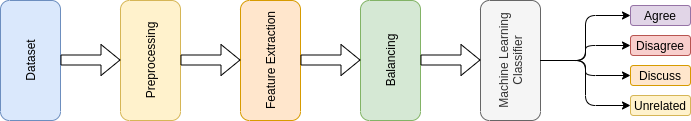
\includegraphics[width=14.5cm]{statistics/schema/ml.png} }
	\caption{Schematic of each machine learning model.}%
	\label{fig:mlschm}%
\end{figure}


\subsection{Gaussian Naive Bayes}
The first machine learning algorithm used to classify stance is Gaussian Naive Bayes Classifier (\cite{GNbayes}). It is an alternative to machine learning Naive Bayes classifier that is inspired by Bayes Theorem\footnote{en.wikipedia.org/wiki/Naive\_Bayes\_classifier}:

\[ P\left(y | X\right) =   \frac{P(X|y).P(X)}{P(y)} \]
where:
\begin{eqexpl}[25mm]
	\item{$X$} List of predictors that are independent of each other.
	\item{$y$} Label of a class.
	\item{$P\left(X|y\right)$} Probability of class with label $y$ from given X predictors.
\end{eqexpl}
 Naive Bayes Classifier algorithm estimates the probability of each class. Gaussian Naive Bayes means that predictors are continuous and follow Gaussian distribution:
 
 \[p\left(x=\upsilon | C_{k}\right) = \frac{1}{\sqrt{2\pi\sigma_{k}^{2}}}e^{-\frac{\left(\epsilon-\mu_{k}\right)^{2}}{2\mu^{2}_{k}}}\]
\begin{eqexpl}[25mm]
	\item{$C_{k}$} Class k.
	\item{$\mu_{k}$} Mean of $x$ values associated with $C_{k}$
	\item{$\sigma^{2}_{k}$} Bessel corrected variance x values associated with $C_{k}$
\end{eqexpl}

\subsection{SVC\protect\footnote{wikipedia.org/Support-vector\_machine}}
\label{SVM}
SVC stands for SVM Classifier. Support Vector Machines (\cite{svc})  are a group of supervised machine learning models. One of their applications is the classification problem. SVM algorithms map each sample to a space such that samples of a particular class locate as far as possible from other classes samples. In other words, SVM is looking for an n-dimensional hyperplane which can separate classes as clearly as possible.

SVC model from \textit{scikit-learn}\footnote{scikit-learn.org/stable/modules/generated/sklearn.svm.SVC.html} python library is used in this project. Regularization parameter ($ c $) which is stands for strength of regularization is tuned depends on task. As the kernel three different \textit{rbf}, \textit{sigmoid}, and \textit{poly} hyperplane are evaluated. Kernel specifies the type of separator that SVM algorithm uses to distinguish different classes. Furthermore, \textit{class\_weight} parameter set to \textit{balanced} which mean set different weight for each class during training to compensate imbalanced data. 


\subsection{LinearSVC}
LinearSVC is an alternative algorithm for SVC in large datasets. LinearSVC linearly separates samples. Depends on the dataset, it may work better than nonlinear SVC. This model is the same as SVC from the previous part, the only difference is to set \textit{kernel} parameter equal to linear. 
 
\subsection{Random Forest}
Random Forest (\cite{randomforest}) is a machine learning algorithm to deal with complex classification problems. It constructs of many decision trees. The point is that it is more robust than decision threes. Besides Random Forest classifier doesn't need parameter tuning. Each decision three has its own prediction and the final prediction of the model is calculated bt majority voting of each tree output. 

In this project, implemented Random Forest algorithm from \textit{scikit-learn}\footnote{scikit-learn.org/stable/modules/generated/sklearn.ensemble.RandomForestClassifier.html} python library is used. Three parameters of \textit{max\_features} (Maximum number of features allowed to use for each tree), \textit{estimator} (Number of decision trees), and \textit{criterion} (Algorithm to measure quality of splits in nodes) are tuned for the desired task.

\subsection{Logistic Regression}
Logistic Regression is a machine learning classification algorithm. Its functionality is mainly for Binary Classification. In multi-class datasets, logistic regression classifies one class vs rest. This algorithm uses Sigmoid function as its cost function and its prediction is based on probabilities. 

Implemented Logistic Regression algorithm from \textit{sckiti-learn}\footnote{scikit-learn.org/stable/modules/generated/sklearn.linear\_model.LogisticRegression.html} python library is used. \textit{penalty} parameter could be chosen from \textit{l1} (Equation \ref{eq:logil}), \textit{l2} (Equation \ref{eq:logill}), and \textit{elasticnet} (Equation \ref{eq:logisel}) for penalization and regularization.
\begin{itemize}
	
	\item $l1$
		\begin{equation}
		\label{eq:logil}
		 min_{\omega,c} \; \frac{1}{2}\omega^{T}\omega + C \Sigma_{i=1}^{n} \log\left(\exp\left(-y_{i}\left(X^{T}_{i}\omega + c \right)\right) + 1 \right)
		\end{equation}
	\item $l2$
		\begin{equation}
		\label{eq:logill}
		 min_{\omega,c} \; \left|\left|\omega\right|\right|_{1} + C \Sigma_{i=1}^{n} \log\left(\exp\left(-y_{i}\left(X^{T}_{i}\omega + c \right)\right) + 1 \right) 
		\end{equation}
		
	\item $elastic-net$
		\begin{equation}
		\label{eq:logisel}
		min_{\omega,c} \; \frac{1-\rho}{2}\omega^{T}\omega +\rho\left|\left|\omega\right|\right|_{1} + C \Sigma_{i=1}^{n} \log\left(\exp\left(-y_{i}\left(X^{T}_{i}\omega + c \right)\right) + 1 \right) 
		\end{equation}
	
\end{itemize}
where:
\begin{eqexpl}[25mm]
	\item{$\rho$} Controls $\; l1 \;$ strength (\textit{l1\_ration} parameter).
	\item{$y_{i}$} Takes value between -1, 1.
\end{eqexpl}
\bigbreak
Elastic-Net Penalization is used with $\; \rho \;$ parameter equals to 0.5, means $\;l1\;$ and $\;l2\;$ have the same powers and \textit{solver} parameter which stands for optimizer algorithm is set to \textit{sega} which is an alternative for Stochastic Average Gradient (sag) optimizer. 

Another optimization algorithm for Logistic Regression such as \textit{sag}, \textit{lbfgs}, and \textit{liblinear} are also evaluated. In this setup, penalization is set to $\; l2$. \textit{lbfgs} optimizer performs more robust in larger datasets. Although, it is slower than \textit{saga}\footnote{scikit-learn.org/stable/modules/linear\_model.html\#logistic-regression}. 

\section{Balancing}
As mentioned in section \nameref{sec:dataset}, Figure \ref{fig:datacom}, the number of samples in dataset classes was imbalanced. As a result, models bias on majority class and there may not enough sample in minority class for a model to learn that, this leads to having high accuracy score (Equation \ref{eq:acc}) while having low f1 score (Equation \ref{eq:f1}).  
\begin{equation}
\label{eq:acc}
F1 = \frac{TP + TN }{TP + FN + TN + FP}
\end{equation}
where:
\begin{eqexpl}[25mm]
	\item{$TP$} True Positive
	\item{$TN$} True Negative
	\item{$FP$} False Positive 
	\item{$FN$} False Negative
\end{eqexpl}

\begin{equation}
	\label{eq:f1}
	 F1 = \frac{2 \times precision \times recall }{precission + recall}
\end{equation}
where: 
\begin{eqexpl}[25mm]
	\item{$precission$} $\; precision = \frac{TP}{TP + FP} \;$
	\item{$recall$} $\; recall = \frac{TP}{TP + FN} \;$ 
\end{eqexpl}

\bigbreak
There are several algorithms to deal with imbalanced datasets. In \cite{stance_persian} minority class forms only 7.4\% of data (Figure \ref{fig:datacom}). So it's not practical to rely on only one method and except to perform in the best way. Consequently, three different methods were used in this project in order to deal with this phenomenon. Methods of balancing a dataset which is used in this project are described in the following sections.  
	
\subsection{Extending dataset}
The simplest method is to gather data for classes except for the majority class. But unfortunately, it is not always practicable. Another way of extending a dataset is to use another existing dataset which has similar gathering logic and it is possible to map these two dataset classes. 

ParsFEVER (\cite{parsfever}) is a Persian dataset set based on FEVER (\cite{fever}) dataset is gathered for fact extraction and verification task. \cite{parsfever} claims are generated from Wikipedia\footnote{wikipedia.org} articles manually, then pieces of evidence for each claim are extracted from Wikipedia separately by distinct annotators. This dataset contains three \textit{Support}, \textit{Refute}, and \textit{Not Enough Info} classes. 
\begin{itemize}
	\item {\color{green!70!black}\textbf{Support:}} The article obviously proves the given claim. 
	\item {\color{red!60!black}\textbf{Refute:}} The article obviously disproves the given claim.
	\item {\color{gray}\textbf{Not Enough Info:}} There isn't enough information in the article about the claim. 
\end{itemize}                

According to Figure \ref{fig:datacom} two \textit{Agree} and \textit{Disagree} class in \cite{stance_persian} dataset suffers from lack of samples. In this project, \textit{Supports} and \textit{Refutes} samples from \cite{parsfever} dataset are mapped to \textit{Agree} and \textit{Disagree} class of \cite{stance_persian} dataset respectively. 
But it is not possible to extend \textit{Discuss} or \textit{Unrelated} class by ParsFEVER, because they are both merged in \textit{Not Enough Info} class. As a result, two \textit{Agree} and \textit{Disagree} extended as much as possible with random selected samples from ParsFEVER dataset. Sample distribution is illustrated in figure \ref{fig:datab1}. Dataset is still imbalanced in one class for both Article to Claim and Headline to Claim.

\begin{figure}%
	\centering
	\subfloat[\centering Artcile to Claim]{{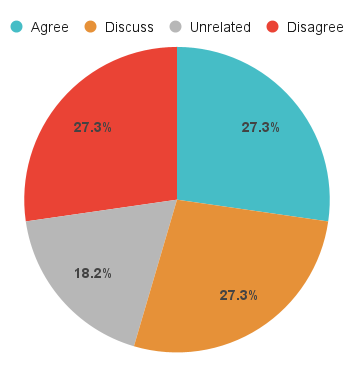
\includegraphics[width=6cm]{statistics/stance/a2c_b1.png} }}%
	\qquad
	\subfloat[\centering Headline to claim ]{{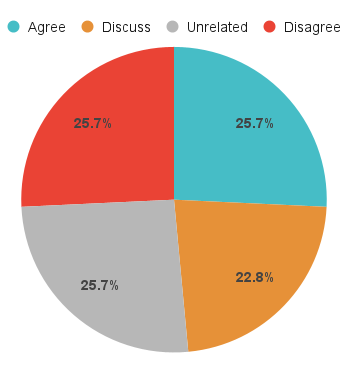
\includegraphics[width=6cm]{statistics/stance/h2c_b1.png} }}%
	\caption{Comparison between Article to claim and Headline to claim labels, samples distribution in \cite{stance_persian} dataset, after extending by \cite{parsfever} .}%
	\label{fig:datab1}%
\end{figure}

\subsection{Oversampling and Undersampling}
 Another common way of dealing with an imbalanced dataset is automatically augmenting samples to achieve balanced class distribution (Oversampling) or even reduce the number of samples in the majority class (Undersampling). Undersampling is applicable on a large dataset. But in small datasets, it's not wise to ignore some samples. Oversampling methods suites for such datasets. According to figure \ref{fig:datacom}, oversampling should be performed classes except the majority class. It is important to split test and train sets before resampling, and oversampling should be only apply on the train set. Resampling methods that were evaluated are: 
\begin{itemize}
	\item \textbf{RandomOverSampler\footnote{imbalanced-learn.org/stable/references/generated/imblearn.over\_sampling.RandomOverSampler.html}:} This method randomly peak samples from classes and resample them. Random Over Sampler is the most naive algorithm and its performance is same as increasing minority class loss weight. Another variant of this method is smoothed bootstrap oversampling. It is generally similar to Random Oversampler, but new samples don't exactly overlap original samples. They are adjacent to source samples. This variant can be implement by \textit{shrinking} parameter in \textit{RandomOverSampler} from \textit{imblearn} python library. 
	
	\item \textbf{SMOTE:} 
	Synthetic Minority Over-sampling Technique (\cite{smothe}) is an oversampling method by generating new samples by interpolation. It's not important for smothe sampler that point is chosen to be resampled. 
	
	\item \textbf{SVMSMOT\footnote{imbalanced-learn.org/stable/references/generated/imblearn.over\_sampling.SVMSMOTE.html}:} 
	SVMSMOTE (\cite{svmsmothe}) is a variant of SMOTE oversampling method which uses SVM (Section \ref{SVM}) algorithm to choose resampling samples. One strength of this model is that it is effective for both vector data and sequence data (\cite{svmsmothe}).
	
	\item \textbf{BorderlineSMOTE\footnote{imbalanced-learn.org/stable/references/generated/imblearn.over\_sampling.BorderlineSMOTE.html}:} 
	BorderlineSMOTE (\cite{borderlinesmothe}) is also another variant of SMOTE oversampler. Borderline samples are mainly chosen to get resample in this variant. \cite{borderlinesmothe} has achieved better accuracy than SMOTE.
	\item \textbf{ADASYN\footnote{imbalanced-learn.org/stable/references/generated/imblearn.over\_sampling.ADASYN.html}:} 
	Adaptive Synthetic Sampling Approach for Imbalanced Learning (\cite{adasyn}) focuses on generating new samples adjacent to those samples wrongly classified by employing K-Nearest Neighbors classifier. These samples are considered as hard samples because it's not easy for models to predict them, as a result, ADASYN increases the robustness of the desired dataset. This method performs better in comparison to Decision Tree and SMOTE algorithms (\cite{adasyn}). In this project number of nearest neighbors to generate a new sample is set to 9.
	
\end{itemize}
All mentioned oversampling methods are evaluated against each other in this project and utilized from oversampling package of \textit{imblearn} \footnote{imbalanced-learn.org/stable/references/over\_sampling.html} python library. 

\subsection{Tune mode parameters}
 The last but not least important balancing method is to choose a robust learning algorithm for an imbalanced dataset, Choosing a weight of each class according to the ratio of samples of each class and choosing an optimizer and loss function that can overcome an imbalanced dataset. After applying previous methods to balance the dataset, this step can be skipped in this project. 




\section{Deep Learning}
In deep learning approach, a combination of all predictors can be fed into the model and the model on its own will automatically learns which predictor is useful for the task. This property is the biggest advance of deep learning in comparison to machine learning (\cite{book_datafake}). In contrary, in machine learning it was a critical step to design input predictors that the model can performs the best. And hours of trying different combination of predictors is needed (\cite{book_fake}). \cite{stance_robust} assessed that, In contrast deep learning models, machine learning models that is trained on a single dataset, usually generalize poorly to other domains.

\begin{figure}% 
	\centering
	{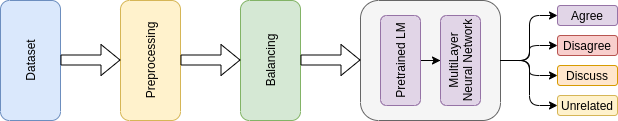
\includegraphics[width=14.5cm]{statistics/schema/dl.png} }
	\caption{Schematic of each machine learning model.}%
	\label{fig:dlschm}%
\end{figure}

\subsection{BERT}
ParsBERT (\cite{ParsBERT}) pre-trained model is used at the top of the model. ParsBERT model is a monolingual transfromer language model based on Google's BERT model \cite{bert}. Pretrained BERT model is adopt from HooshvareLab\footnote{\href{https://huggingface.co/HooshvareLab}{huggingface.co}}. BERT is used to extract in context features from the corpus. Input of the model are \textit{input ids}, \textit{token type ids}, and \textit{attention mask}. Then, two dense layer and another dense layer as the classifier is added to the output of the BERT model. 

\subsection{ALBERT}
In this experiment, ALBERT (\cite{albert})	 model is substitute with BERT model in figure \ref{fig:deepshema}.  Other configurations are same as BERT experiment.

\section{Article to Claim}
Deep learning models perform far better on language inference tasks so they are better choices for article-to-claim stance classification. To calculate stance of a claim toward the body of a news, three different model based on a pre-trained Persian language model based on BERT, ParsBERT, and  ALBERT are evaluated against each other. 

\section{Fake News Detection}
To detect a news article veracity, headline-to-claim and article-to-claim stance detection models, are considered as a black box. Four news articles is considered to evaluate veracity of a claim. Firstly, stance of a claim toward each headline of desired news articles and the body of the news article predict by stance classifier models. All predicted stance vectors are concatenated and along with some other features are fed into a multi-layer perception network in order to predict the claim veracity.

Credibility of news websites is one of the most important extracted feature. The credibility can be calculated through the following steps (The credibility score of head-claim and article-claim is calculated similarly except using their related stance ground truth):

\begin{itemize}
	\item \textbf{Initialization}: The credibility score of all news websites that are existing in the \cite{stance_persian} dataset is set to zero at first. For the test set or predicting new samples, if the website doesn't exist in the data set, credit score is set to 0.1.


	\item \textbf{Quantification:}
	For each sample in the dataset, credibility score changes according to Table \ref{tbl:cred}. $\rho$ value is calculated from equation \ref{eq:cred} if it is needed.
	\begin{table}[H]
		\centering
		\caption{Value of credibility according to GroundTruth and Veracity labels. }
		\setlength{\extrarowheight}{13pt}%
		\begin{tabular}{|l|l|l|}
			\hline
			GroundTruth & Veracity & Value \\
			\hline
			Agree       & True     & $+1$    \\
			\hline
			Disagree    & False    & $+1$    \\
			\hline
			Agree       & False    & $-1$    \\
			\hline
			Disagree    & True     & $-1$    \\
			\hline
			Discuss     & True     & $+\rho$    \\
			\hline
			Discuss     & False    & $-\rho$   \\
			\hline
			Unrelated     & -   & No change   \\
			\hline
			-     & Discuss    & No change   \\
			\hline
		\end{tabular}
		\label{tbl:cred}
	\end{table}

	\begin{equation}
	\label{eq:cred}
	\rho = \frac{P(x,Agree) - P(x,Disagree)}{P(x,Agree) + P(x,Disagree)}\\
	\end{equation}

where: 
\begin{eqexpl}[25mm]
\item{$P(x,Agree)$} Probability of Agree
\item{$P(x,Disagree)$} Probability of Disagree 
\end{eqexpl}
	
	\item \textbf{Score Calculation:} The credibility score for each news website is calculated from equation \ref{eq:honesty}.
	\begin{equation}
	\label{eq:honesty}
	H(X) = \frac{\sum_{i=1}^{k_{X}} credibility\,of\,x_{i}}{k_{X}}
	\end{equation} 
	where:
	\begin{eqexpl}[25mm]
		\item{$X$} A news website
		\item{$k_{x}$} The number of news article in the dataset from x
		\item{$credibility\,of\,x_{i}$} Due to table \ref{tbl:cred}
	\end{eqexpl}

\end{itemize}


Also another features are extracted to detect fake news, such as :
\begin{itemize}
	\item One-hot encoding of the news website domain
	\item The ratio of samples that have been properly labeled as agree or disagree to the total sample of the news website (Correct ratio)
	\item The ratio of samples that have been wrongly labeled as agree or disagree to the total sample of the news website (Wrong ratio)
	\item The ratio of the total number of news website articles to the total number of articles in the data set.	
\end{itemize}



